\documentclass[12pt,letterpaper]{article}

% --- Paquetes Requeridos ---
\usepackage[utf8]{inputenc}
\usepackage[spanish,es-tabla]{babel}
\usepackage[margin=2.5cm]{geometry}
\usepackage{graphicx}
\usepackage{float}
\usepackage{titlesec}
\usepackage{setspace}
\usepackage{hyperref}
\usepackage{booktabs}
\usepackage{caption}
\usepackage{enumitem}
\usepackage{listings}
\usepackage{xcolor}

% --- Configuración de Párrafo ---
\onehalfspacing
\setlength{\parindent}{0pt}
\setlength{\parskip}{1em}

% --- Rutas de búsqueda de imágenes ---
% Permite compilar tanto desde Documentos/Entregables/ como con todas las
% imágenes en una sola carpeta plana.
\graphicspath{{./}{../Evidencia/}{Evidencia/}{imagenes/}}

% --- Configuración de listings ---
\lstset{
    basicstyle=\ttfamily\footnotesize,
    breaklines=true,
    frame=single,
    captionpos=b,
    showstringspaces=false
}

% --- Inicio del Documento ---
\begin{document}

% --- PORTADA ---
\begin{titlepage}
    \centering

    {\Large \textbf{UNIVERSIDAD SANTO TOMÁS}} \\[1cm]

    {\Large \textbf{Sistema colaborativo de robots móviles para asistencia de orientación en entornos interiores con múltiples pisos}} \\[2cm]

    {\large \textbf{Realizado por:}} \\
    {\large Santiago Hernández Ávila} \\
    {\large Jonny Alejandro Mejía León} \\[1cm]

    \begin{figure}[H]
        \centering
        \includegraphics[width=0.6\textwidth]{Logos Uni.png}
        \label{Logo Universidad Santo Tomas y facultad de ingenieria electronica}
    \end{figure}

    \vfill

    {\large \textbf{Informe de Avance --- Semana 25}} \\
    {\large Fase 5: integración del sistema y realización de pruebas} \\
    {\large Pruebas de odometría y navegación en el edificio} \\[1.5cm]

    \textbf{Dirigido por:} \\
    Ing. Armando Mateus Rojas, Msc. \\
    Ing. Nestor Ivan Ospina, Msc. \\
    Ing. Oscar Mauricio Gélvez Lizarazo, Msc. \\[1.0cm]

    \vfill

    {\large GED (Grupo de Estudio y Desarrollo en Robótica)} \\
    {\large Facultad de Ingeniería Electrónica} \\
    {\large División de Ingenierías} \\
    {\large Bogotá, octubre de 2026}
\end{titlepage}

% --- CONTENIDO ---

\section{Introducción}

Este informe presenta el avance de la semana 25 del cronograma (28 de septiembre al 4 de octubre de 2026, con corte el viernes 2), dentro de la fase 5, integración del sistema y realización de pruebas.

La semana se dedicó a las compuertas G-2 y G-3, que el acta de la decisión GO/NO-GO exigía para el primer corte, C-1, el viernes 2 de octubre. G-2 evalúa la odometría, la estimación del desplazamiento del vehículo; G-3, la navegación de un vehículo con Nav2, el sistema de navegación de ROS~2. Las compuertas son condiciones verificables, cada una con su fecha, que deben cumplirse para continuar con la demostración física; los cortes son las fechas en que se revisan.

Los dos vehículos quedaron aislados entre sí y se probaron en tres sitios. En el hall del piso 2 el modelo del edificio no correspondía a las medidas reales. El equipo levantó entonces con flexómetro los pisos 3 y 4, que los directores y los evaluadores aprobaron como sitio nuevo el 2 de octubre. En el piso 4, la odometría cumplió el criterio de G-2 en las dos corridas medidas; la llegada no cumplió el de G-3. La Tabla~\ref{tab:compuertas} resume el estado de las compuertas.

\begin{table}[H]
    \centering
    \small
    \caption{Compuertas del acta GO/NO-GO al 4 de octubre.}
    \label{tab:compuertas}
    \begin{tabular}{@{}p{3.4cm}p{5.6cm}p{5.0cm}@{}}
        \toprule
        \textbf{Compuerta} & \textbf{Qué exige} & \textbf{Estado al 4 de octubre} \\ \midrule
        G-1, actuación & El vehículo responde a las órdenes de dirección y tracción & Alcanzada el 22 de septiembre \\ \addlinespace
        G-4, coexistencia & Los dos vehículos y el coordinador (el programa que asigna las misiones y organiza el relevo) en la misma red, sin conflicto de nombres & Alcanzada el 22 de septiembre \\ \addlinespace
        G-2, odometría & Error de hasta 10~\% sobre un recorrido medido de al menos 5~m & Criterio cumplido en las dos corridas medidas del piso 4 (+3,3~\% y $-$4,6~\%); falta declararla en el acta \\ \addlinespace
        G-3, navegación de un vehículo & Un recorrido de punto a punto con Nav2, con la llegada verificada & No alcanzada: llegadas a 0,57~m y 0,62~m, con tolerancia de 0,5~m \\ \addlinespace
        G-5, protocolo completo & Una misión (guiar a un usuario de un origen a un destino) con relevo entre los dos vehículos, uno en cada piso & Pendiente \\ \addlinespace
        G-6, RF-27 & Las repeticiones de RF-27 con el protocolo completo & Pendiente; requiere G-5 \\ \bottomrule
    \end{tabular}
\end{table}

\section{Objetivos de la semana}
\label{sec:objetivos}

El cronograma fija para esta semana el siguiente criterio de cierre:

\begin{quote}
\textit{Corridas físicas registradas con la misma instrumentación que en simulación; video de la demostración listo.}
\end{quote}

El criterio no se cumplió. El 25 de septiembre, al replanificar la semana contra las fechas del acta, la campaña de RF-27 pasó a la semana 27, porque exige el protocolo completo con los dos vehículos (G-5). La semana 25 quedó para las compuertas G-2 y G-3 y para montar el sistema en los vehículos (\texttt{PLAN\_S25.md}). De ese plan se cumplieron el aislamiento de los vehículos, las decisiones del director y la configuración con espacios de nombres en el portátil; G-2 se midió y G-3 no se alcanzó.

\section{Decisiones del director}
\label{sec:decisiones}

El 28 de septiembre, el director, Ing. Armando Mateus Rojas, resolvió los puntos siguientes, que quedaron en la sección 6.1 del acta:

\begin{enumerate}[leftmargin=*]
    \item La demostración física se hace en los pasillos reales del edificio, los mismos que modela la simulación.
    \item El número de repeticiones de RF-27 no se fija por adelantado; se elige con los resultados de las primeras corridas del sistema completo.
    \item La tolerancia de llegada pasa de 0,25~m a 0,5~m en los vehículos reales. La campaña en simulación conserva 0,25~m.
\end{enumerate}

\section{Aislamiento de los dos vehículos}
\label{sec:aislamiento}

Con los dos vehículos encendidos, una orden de movimiento llegaba a los dos y la odometría de cada uno recibía el LiDAR (el sensor láser que mide las distancias alrededor del vehículo) del otro. Los tópicos del software del fabricante, que son los canales por los que se publican esos mensajes, no llevan espacio de nombres. El 28 de septiembre se instaló en cada vehículo una partición de comunicaciones propia: una configuración de la capa de comunicaciones de ROS~2 que hace que cada vehículo intercambie esos mensajes solo con los procesos de su misma partición. Las cinco pruebas pasaron en los dos vehículos (Tabla~\ref{tab:aislamiento}).

\begin{table}[H]
    \centering
    \small
    \caption{Pruebas del aislamiento entre los dos vehículos.}
    \label{tab:aislamiento}
    \begin{tabular}{@{}p{7.0cm}p{7.0cm}@{}}
        \toprule
        \textbf{Prueba} & \textbf{Resultado} \\ \midrule
        La partición funciona en ROS~2 Jazzy, la versión de los vehículos & 9 de 9 comprobaciones en cada vehículo \\ \addlinespace
        El software del fabricante arranca con su partición & Sí, en los dos \\ \addlinespace
        El LiDAR solo se recibe con la partición & 6,97~Hz y 6,71~Hz con ella; ningún barrido sin ella \\ \addlinespace
        Una orden de dirección solo mueve su vehículo & Sí, en los dos \\ \addlinespace
        Con los dos encendidos, cada odometría recibe solo su LiDAR & 7,14~Hz y 6,70~Hz, frente a 14,68~Hz mezclados el 23 de septiembre \\ \bottomrule
    \end{tabular}
\end{table}

El 29 de septiembre se encontró que la imagen de la cámara de cada vehículo también llegaba al otro por la red inalámbrica, unos 1~MB/s en cada sentido, y se incluyó en la partición.

\section{Ajustes de la navegación en el vehículo}
\label{sec:ajustes}

Los ensayos del 29 y el 30 de septiembre dejaron varios ajustes propios del vehículo real. Están en la configuración de Nav2 y en los programas que le dan los datos y mueven el vehículo. Los principales son estos:

\begin{itemize}[leftmargin=*]
    \item La tarjeta de dos núcleos no sostiene el controlador a 20~Hz; se fijó en 10~Hz, y el plazo del gestor que vigila los programas de Nav2 pasó de 4~s a 20~s.
    \item El controlador de tracción no movía el vehículo con órdenes por debajo de 0,40~m/s. Desde el 29 de septiembre esas órdenes salen con el escalón más bajo que sí lo mueve.
    \item rf2o, el paquete que estima la odometría a partir de barridos consecutivos del LiDAR, leía la posición del sensor una sola vez al arrancar. Si en ese momento no estaba disponible, la odometría salía invertida, porque el LiDAR va montado a 180$^\circ$. Se corrigió con una modificación de cuatro líneas al paquete, instalada en los dos vehículos.
    \item Nav2 da la meta por alcanzada a 1,0~m, y no a 0,25~m. Con 0,25~m el vehículo llegaba cerca de la meta y retrocedía buscándola, porque con dirección de tipo Ackermann no puede corregir en un espacio tan corto. Ese margen es el punto en que Nav2 deja de mover el vehículo; la llegada se sigue midiendo con flexómetro contra 0,5~m.
\end{itemize}

En una recta de 3,39~m medida con flexómetro, la odometría registró 3,458~m, un 2,0~\% de más.

\section{Pruebas en el hall del piso 2}
\label{sec:piso2}

El 30 de septiembre se hicieron las primeras pruebas en el edificio, en el hall del extremo oeste del piso 2, con el vehículo \texttt{amss-jgm9} y el mapa que se genera del modelo de la simulación. Por el alcance de la red inalámbrica, las rutas se limitaron a tres destinos: el IEEE, el Laboratorio de Sistemas 313 y las escaleras.

Las medidas de una corrida mostraron que el hall mide 3,40~m de ancho y el modelo daba 4,24~m. Se corrigió el modelo y se regeneró el mapa. Con el mapa corregido, AMCL (el método de localización sobre el mapa, basado en un filtro de partículas) acertó de lado (0,15~m), pero a lo largo del hall acumuló hasta 2,62~m de error. La odometría registró el 73~\% del recorrido medido en las dos corridas hacia las escaleras, y las dos llegadas quedaron a 1,43~m y 1,26~m del destino (Figura~\ref{fig:piso2}). El vehículo terminó a 0,55~m y 0,25~m del borde de la escalera, así que se suspendió la navegación hacia ella.

\begin{figure}[H]
    \centering
    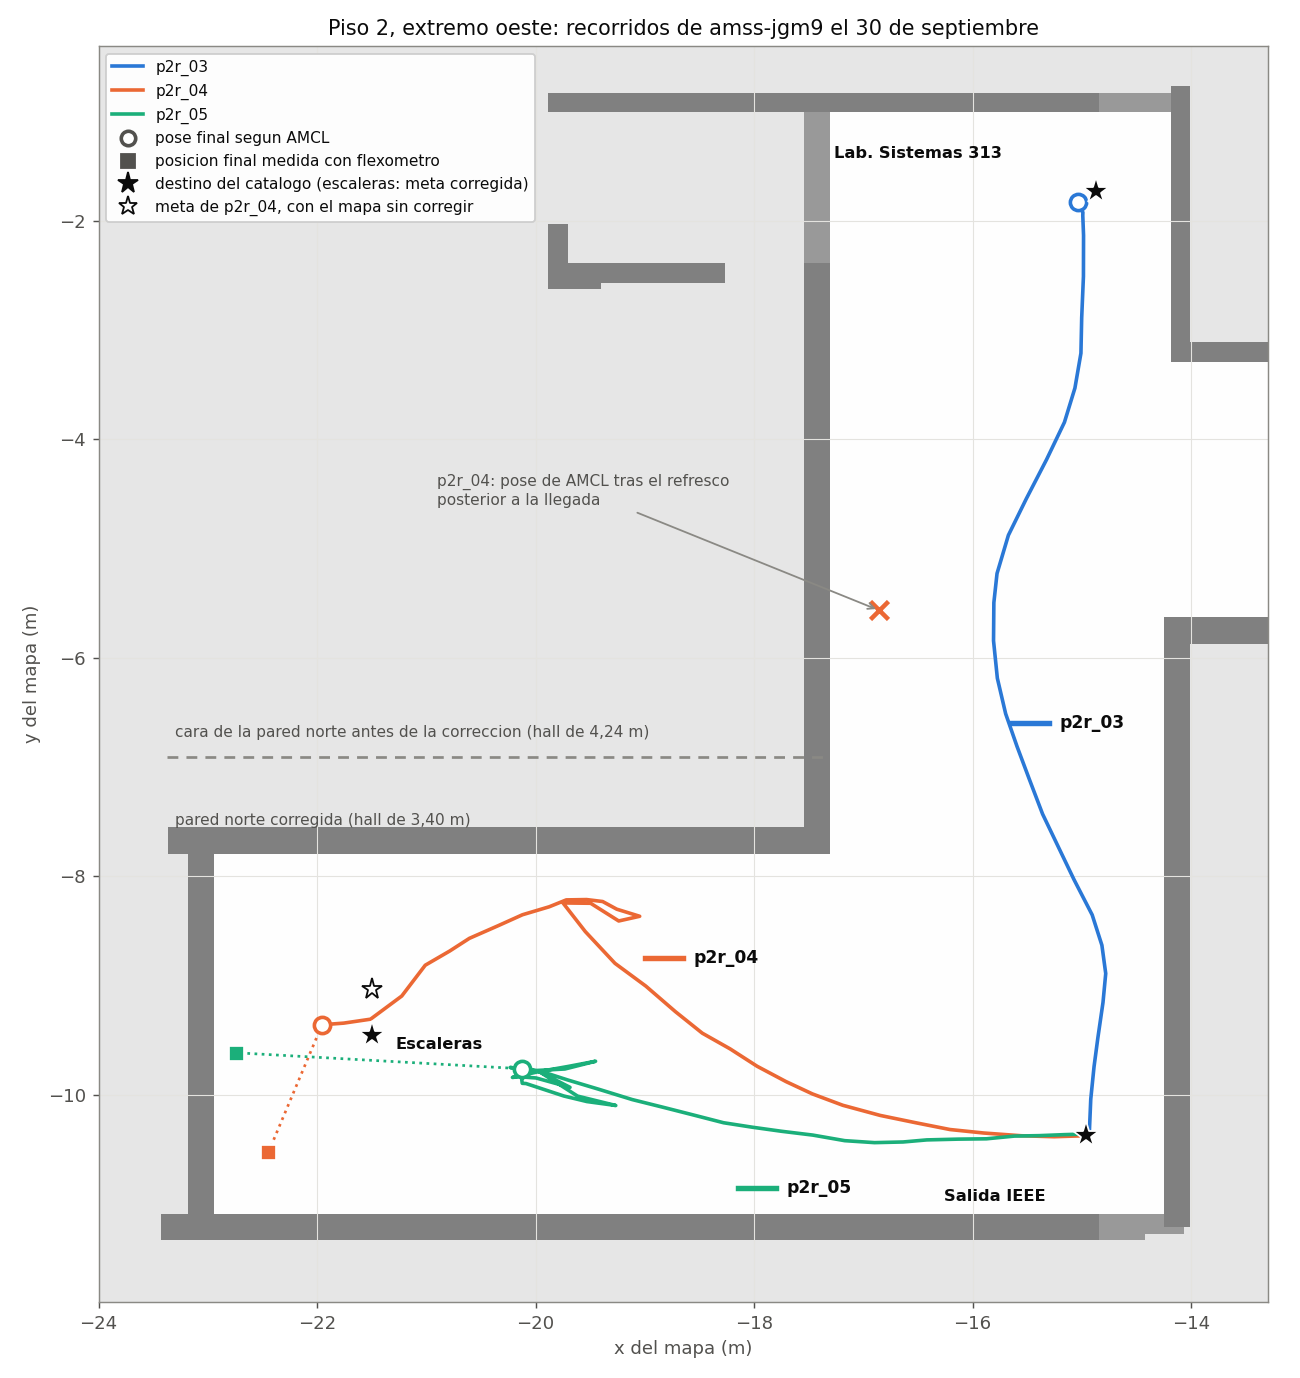
\includegraphics[width=0.85\textwidth]{S25_p2_recorridos_hall.png}
    \caption{Recorridos según AMCL en el hall del piso 2, sobre el mapa corregido, con la pose final de AMCL y la posición medida con flexómetro. En las corridas hacia las escaleras, AMCL situó al vehículo hasta 2,6~m antes de su posición real.}
    \label{fig:piso2}
\end{figure}

\section{Cambio de sitio a los pisos 3 y 4}
\label{sec:sitio}

El ancho del hall del piso 2 era la primera medida del modelo comprobada con flexómetro, y el modelo lo daba un 25~\% mayor que el real. Las demás medidas del modelo nunca se habían comprobado. Jonny Mejía levantó con flexómetro los pasillos de los pisos 3 y 4 y generó de ese levantamiento el modelo de la simulación y el mapa de navegación a la vez, de modo que los dos coinciden con el edificio. Al recorrer cada piso por sus dos paredes, el levantamiento cierra con un error de 0,32~\% en el piso 4 y de 0,62~\% en el piso 3, dentro del 2~\% que se fijó como criterio. Cada piso tiene cinco destinos: tres salones, el ascensor y las escaleras.

El 2 de octubre los directores y los evaluadores aprobaron el cambio de sitio. Falta registrarlo en la sección 6.1 del acta.

\section{Pruebas en el piso 4}
\label{sec:piso4}

El 2 de octubre se hicieron cinco corridas en el piso 4 con los dos vehículos, cuatro de ellas desde las escaleras hacia los salones. Dos se midieron con flexómetro (Tabla~\ref{tab:piso4}).

\begin{table}[H]
    \centering
    \small
    \caption{Corridas del piso 4 medidas con flexómetro.}
    \label{tab:piso4}
    \begin{tabular}{@{}lllcccc@{}}
        \toprule
        \textbf{Corrida} & \textbf{Vehículo} & \textbf{Destino} & \textbf{Medido} & \textbf{Odometría} & \textbf{Error} & \textbf{A la meta} \\ \midrule
        p4r\_03 & \texttt{amss-jgm9} & Salón 403 & 6,68~m & 6,370~m & $-$4,6~\% & 0,62~m \\
        p4d\_01 & \texttt{amss-ez9n} & Salón 402 & 14,57~m & 15,045~m & +3,3~\% & 0,57~m \\ \bottomrule
    \end{tabular}
\end{table}

La odometría cumplió el criterio de G-2 en las dos corridas, y es la primera vez que lo hace en un pasillo del edificio. La corrida p4d\_01 es la medida más limpia: 14,57~m, con la salida medida desde dos paredes y sin tocar el vehículo. En p4r\_03 la salida no quedó exacta y el vehículo tuvo que ser empujado para arrancar.

Las dos llegadas quedaron cortas, a 0,57~m y 0,62~m de la meta (Figura~\ref{fig:piso4}). Al detenerse, AMCL situaba los vehículos a 0,96~m y 0,74~m de la meta, dentro del margen de 1,0~m en que Nav2 la da por alcanzada. El error de AMCL frente a la posición medida fue de 0,42~m y 0,43~m, frente a los 2,62~m del hall del piso 2.

\begin{figure}[H]
    \centering
    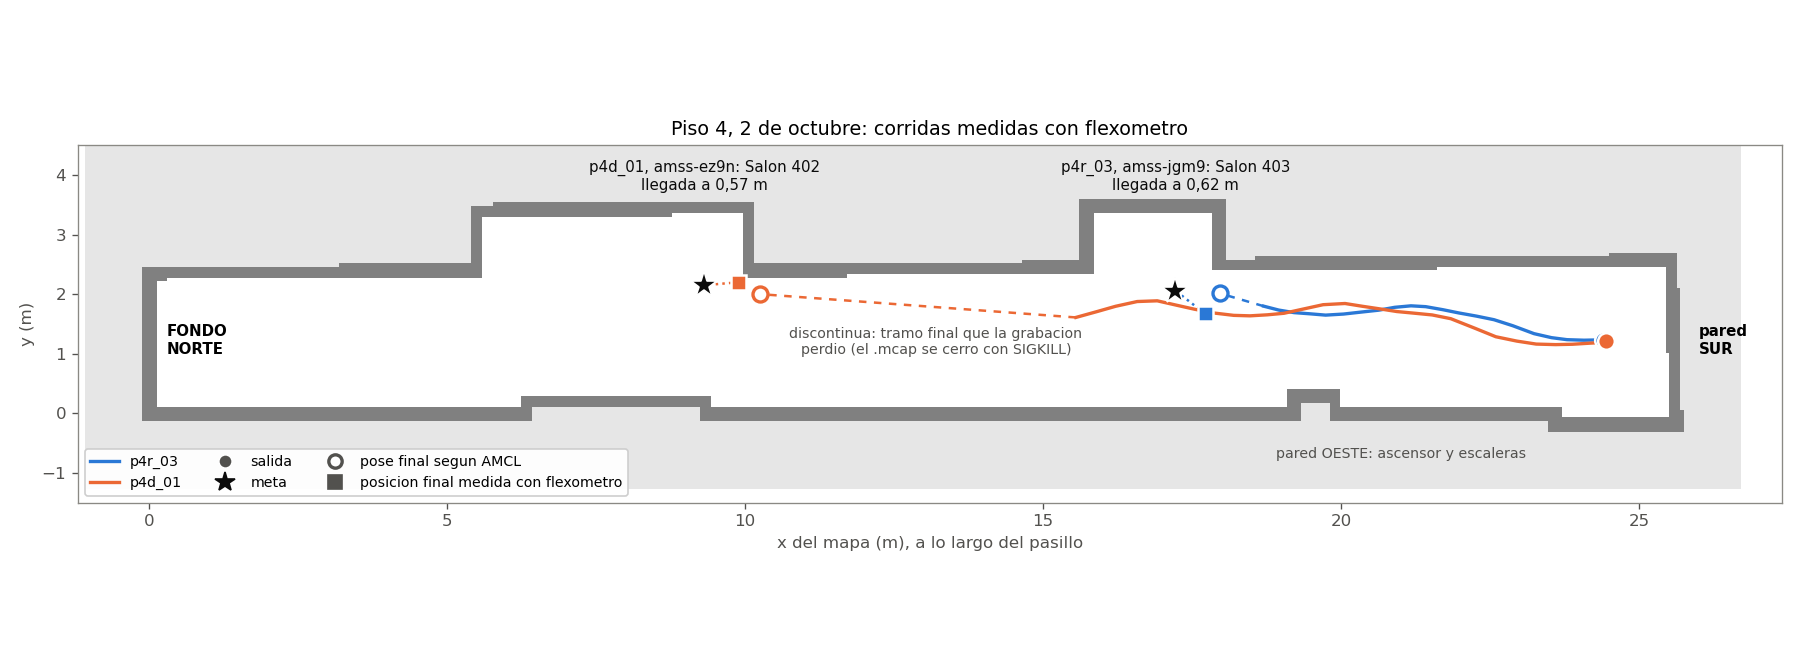
\includegraphics[width=\textwidth]{S25_p4_corridas_piso4.png}
    \caption{Corridas p4r\_03 y p4d\_01 en el piso 4: recorrido según AMCL, pose final de AMCL y posición final medida con flexómetro. El tramo final de cada recorrido no quedó en la grabación.}
    \label{fig:piso4}
\end{figure}

Las otras tres corridas no llegaron, por causas de operación y no del mapa:

\begin{itemize}[leftmargin=*]
    \item En la primera, Nav2 se desactivó porque la tarjeta del vehículo alcanzó una carga de 22 con la cámara y la fusión de sensores del fabricante encendidas, que el proyecto no usa. Al apagarlas, la carga bajó a 8,6 y Nav2 no volvió a desactivarse.
    \item En otra, Nav2 no obtuvo la posición del vehículo y abortó sin moverlo.
    \item La tercera intentó una media vuelta con Nav2 en un pasillo de 2,3 a 2,4~m de ancho y abortó: el planificador supone un radio de giro de 0,35~m, y el radio real del vehículo no se ha medido.
\end{itemize}

Con la misma escala de velocidad, \texttt{amss-jgm9} no arrancó sin ayuda y \texttt{amss-ez9n} llegó a 1,58~m/s. La red inalámbrica dio retardos de hasta 850~ms y desconectó dos veces a \texttt{amss-ez9n}, y \texttt{amss-jgm9} se quedó sin batería en mitad de la sesión.

\section{Aporte a los objetivos específicos}
\label{sec:aporte}

\subsection{Relación entre actividades y objetivos}

\begin{table}[H]
    \centering
    \small
    \caption{Trazabilidad entre las actividades de la semana y los objetivos específicos.}
    \label{tab:trazabilidad}
    \begin{tabular}{@{}p{4.6cm}cp{7.2cm}@{}}
        \toprule
        \textbf{Actividad} & \textbf{Objetivo} & \textbf{Aporte} \\ \midrule
        Aislamiento de los dos vehículos & OE2 & Por primera vez los dos vehículos pueden estar encendidos a la vez sin interferirse \\ \addlinespace
        Ajustes de la navegación en el vehículo & OE2 & Nav2 funciona en el vehículo con la carga real de la tarjeta y sin invertir la odometría \\ \addlinespace
        Pruebas en el hall del piso 2 & OE2, OE4 & Muestran que el modelo del piso 2 no correspondía al edificio y motivan el cambio de sitio \\ \addlinespace
        Levantamiento de los pisos 3 y 4 & OE2, OE4 & Sitio con modelo y mapa comprobados contra el edificio \\ \addlinespace
        Pruebas en el piso 4 & OE2 & Primera medida que cumple el criterio de G-2 en un pasillo del edificio \\ \bottomrule
    \end{tabular}
\end{table}

\subsection{Estado de los objetivos específicos}

\begin{table}[H]
    \centering
    \small
    \caption{Avance por objetivo específico al cierre de la semana 25.}
    \label{tab:objetivos}
    \begin{tabular}{@{}cp{1.8cm}p{5.0cm}p{5.4cm}@{}}
        \toprule
        \textbf{Objetivo} & \textbf{Avance} & \textbf{Aporte de la semana} & \textbf{Pendiente} \\ \midrule
        OE1 & 100~\% & --- & --- \\ \addlinespace
        OE2 & 79~\% & Aislamiento, ajustes de la navegación y G-2 medido & Los dos vehículos navegando a la vez con espacio de nombres, y el coordinador en un vehículo \\ \addlinespace
        OE3 & 100~\% & --- & --- \\ \addlinespace
        OE4 & 89~\% & Sitio comprobado para la campaña física & RF-27, que requiere el protocolo completo \\ \bottomrule
    \end{tabular}
\end{table}

Desde el 30 de septiembre el avance de cada objetivo es el promedio de sus requisitos. Cada requisito cuenta según su estado: verificado, 100~\%; verificado en simulación y con parte de la prueba física, 75~\%; solo en simulación, 50~\%; con preparación sin prueba, 25~\%. Con esa regla, el avance del objetivo 2 pasó de 65~\% a 79~\% y el del objetivo 4 de 85~\% a 89~\%, sin resultados nuevos: es un cambio de método. El promedio de los cuatro objetivos es 92,0~\%, frente al 78,1~\% del calendario (semana 25 de 32). Lo que falta es la parte física del sistema: el relevo entre los dos vehículos y la campaña de RF-27.

\section{Estado del cronograma y trabajo previsto}
\label{sec:cronograma}

\subsection{Cumplimiento del criterio de cierre}

\begin{table}[H]
    \centering
    \small
    \caption{Criterio de cierre de la semana 25 y su evidencia.}
    \label{tab:cierre}
    \begin{tabular}{@{}p{5.4cm}p{6.0cm}p{2.6cm}@{}}
        \toprule
        \textbf{Parte del criterio} & \textbf{Estado} & \textbf{Evidencia} \\ \midrule
        Corridas físicas registradas con la misma instrumentación que en simulación & No cumplida: la campaña de RF-27 se trasladó a la semana 27 el 25 de septiembre & \texttt{PLAN\_S25.md} \\ \addlinespace
        Video de la demostración & No cumplida; se graba con la campaña & --- \\ \bottomrule
    \end{tabular}
\end{table}

\subsection{Corte C-1}

El corte C-1 del 2 de octubre exigía G-2 y G-3. G-2 cumple su criterio en las dos corridas medidas del piso 4, y G-3 no se alcanzó. El acta prevé que, si una de las dos no se alcanza en el corte, se vuelve a NO-GO: RF-27 se declara no alcanzable y la evidencia queda en la campaña de simulación. Al cierre de este informe, la declaración de las compuertas y el registro del cambio de sitio en el acta están pendientes.

\subsection{Trabajo previsto para la semana 26}

Para la semana 26 (5 al 9 de octubre) el equipo prevé:

\begin{enumerate}[leftmargin=*]
    \item Registrar en el acta el cambio de sitio y el estado de G-2 y G-3.
    \item Comprobar si la tarjeta del vehículo incluye una unidad de medición inercial (IMU) con giroscopio. La documentación del fabricante indica un acelerómetro y un giroscopio integrados, y la comunidad del vehículo tiene un controlador para un sensor Bosch BMI160. Si está, se integrará para mejorar la estimación del rumbo, y con ella se podrá reducir el margen de llegada de Nav2, que hoy es de 1,0~m porque la navegación depende solo del LiDAR.
    \item Desconectar las cámaras de los vehículos, que el proyecto no usa, para reducir la carga de la tarjeta, y ajustar la escala de velocidad de cada vehículo.
    \item Repetir las corridas del piso 4 para cerrar G-2 y evaluar G-3.
    \item Preparar la misión con relevo entre los pisos 3 y 4 (G-5): el coordinador en un vehículo, la red entre los dos pisos y el registro de la misión.
\end{enumerate}

La campaña de RF-27 sigue prevista para la semana 27, con cierre de datos el 16 de octubre (corte C-3), y la sustentación para la semana 28 o 29.

\section{Conclusiones}

\begin{enumerate}[leftmargin=*]
    \item Los dos vehículos pueden estar encendidos a la vez sin interferirse: cada uno recibe solo sus órdenes y su LiDAR.
    \item El modelo del piso 2 no correspondía al edificio: el hall mide 3,40~m y el modelo daba 4,24~m. Los pisos 3 y 4, levantados con flexómetro, cierran con un error de 0,32~\% y 0,62~\%.
    \item En el piso 4 la odometría cumplió el criterio de G-2 en las dos corridas medidas, con +3,3~\% sobre 14,57~m y $-$4,6~\% sobre 6,68~m, frente al 73~\% del recorrido que registró en el hall del piso 2.
    \item G-3 no se alcanzó: las llegadas quedaron a 0,57~m y 0,62~m, cortas, porque Nav2 se detiene dentro de su margen de 1,0~m. El error de AMCL en la llegada fue de 0,42~m y 0,43~m.
    \item Las fallas que impidieron más corridas fueron de operación: la carga de la tarjeta, la red inalámbrica, la batería y la escala de velocidad de cada vehículo.
\end{enumerate}

\section{Anexos}

Las cifras de este informe proceden de los registros y documentos de evidencia del repositorio del proyecto, que se listan a continuación. El mismo informe está disponible en Markdown, en \texttt{Entregable\_semana\_25.md}, para leerlo directamente en el repositorio.

\begin{thebibliography}{99}

\bibitem{acta}
S. Hernández Ávila y J. A. Mejía León,
``Acta de decisión GO/NO-GO de la demostración física,''
Repositorio del proyecto, \texttt{Documentos/ACTA\_GO\_NOGO.md}, septiembre de 2026.

\bibitem{plan}
S. Hernández Ávila,
``Plan de la semana 25,''
Repositorio del proyecto, \texttt{Documentos/PLAN\_S25.md}, septiembre de 2026.

\bibitem{aislamiento}
S. Hernández Ávila,
``Aislamiento de los dos vehículos (bloque A),''
Repositorio del proyecto, \texttt{Documentos/Evidencia/S25\_aislamiento\_dos\_carros.md}, septiembre de 2026.

\bibitem{ensayo}
S. Hernández Ávila,
``Ensayo de B0 con \texttt{amss-jgm9},''
Repositorio del proyecto, \texttt{Documentos/Evidencia/S25\_ensayo\_laboratorio.md}, septiembre de 2026.

\bibitem{piso2}
S. Hernández Ávila,
``Sesión de G-2 y G-3 con \texttt{amss-jgm9} en el piso 2,''
Repositorio del proyecto, \texttt{Documentos/Evidencia/S25\_pasillo\_piso2\_amss-jgm9.md}, septiembre de 2026.

\bibitem{guia34}
J. A. Mejía León,
``Guía del sitio nuevo: pisos 3 y 4,''
Repositorio del proyecto, \texttt{Documentos/GUIA\_PISOS\_3\_Y\_4.md}, octubre de 2026.

\bibitem{piso4}
S. Hernández Ávila,
``Primera sesión en los pisos 3 y 4,''
Repositorio del proyecto, \texttt{Documentos/Evidencia/S25\_pisos34\_campo.md}, octubre de 2026.

\bibitem{estado}
S. Hernández Ávila y J. A. Mejía León,
``Tablero de estado del proyecto,''
Repositorio del proyecto, \texttt{ESTADO.md}, octubre de 2026.

\bibitem{cronograma}
S. Hernández Ávila y J. A. Mejía León,
``Cronograma actualizado, semanas 17 a 32,''
Repositorio del proyecto, \texttt{Documentos/CRONOGRAMA\_S17\_S32.md}, agosto de 2026.

\end{thebibliography}

\end{document}
